\documentclass[a4paper,12pt]{article}
\usepackage[utf8]{inputenc}
\usepackage[ngerman]{babel}
\usepackage{hyperref}
\usepackage{xcolor}
\usepackage{graphicx}
\usepackage{geometry}

\geometry{a4paper, margin=0.5in}

\title{Technische Spezifikationen und Analyse der Intel RealSense Depth Camera D455}
\author{}
\date{}

\begin{document}

\maketitle

\begin{center}
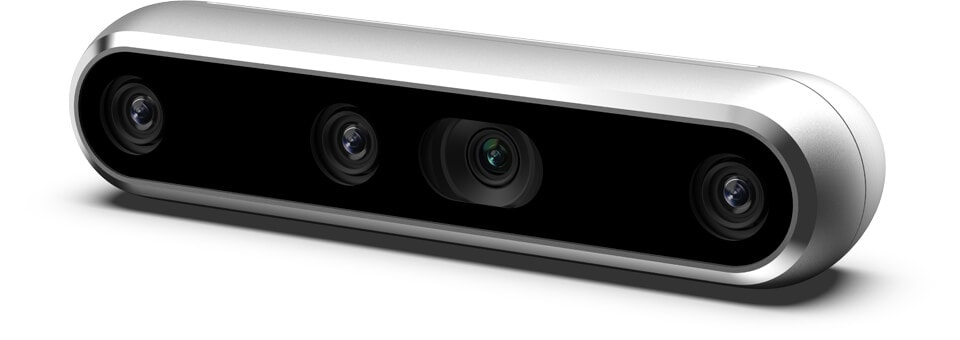
\includegraphics[width=0.8\textwidth]{./Bilder/d455_1.jpg}
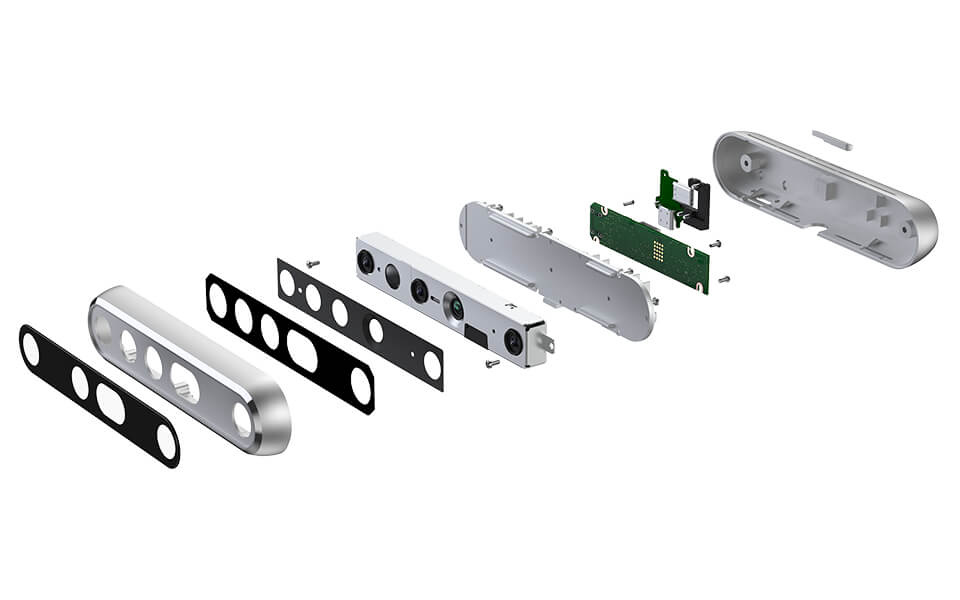
\includegraphics[width=0.8\textwidth]{./Bilder/d455_2.jpg}
\end{center}

\section*{Technische Daten}

\begin{itemize}
    \item \textbf{Tiefensensor:}
    \begin{itemize}
        \item \textbf{Technologie:} Aktive IR-Stereoskopie
        \item \textbf{Auflösung:} Bis zu 1280 × 720 Pixel
        \item \textbf{Bildrate:} Bis zu 90 Bilder pro Sekunde
        \item \textbf{Sichtfeld (FOV):} Horizontal 86°, Vertikal 57°
        \item \textbf{Empfohlener Arbeitsbereich:} 0,6 m bis 6 m
        \item \textbf{Genauigkeit:} Weniger als 2\% Fehler bei 4 m Entfernung
    \end{itemize}
    \item \textbf{RGB-Sensor:}
    \begin{itemize}
        \item \textbf{Auflösung:} 1280 × 800 Pixel
        \item \textbf{Bildrate:} 30 Bilder pro Sekunde
        \item \textbf{Technologie:} Global Shutter
        \item \textbf{Sichtfeld (FOV):} Horizontal 90°, Vertikal 65°
    \end{itemize}
    \item \textbf{Physische Eigenschaften:}
    \begin{itemize}
        \item \textbf{Abmessungen:} 124 mm × 26 mm × 29 mm
        \item \textbf{Gewicht:} 73 g
        \item \textbf{Anschluss:} USB 3.1
    \end{itemize}
    \item \textbf{Besondere Merkmale:}
    \begin{itemize}
        \item \textbf{Integrierte IMU:} Ermöglicht erweiterte Bewegungsverfolgung und Stabilisierung
        \item \textbf{Erweiterter Basisabstand:} 95 mm Abstand zwischen den Tiefensensoren für höhere Genauigkeit
        \item \textbf{Einsatzbereich:} Geeignet für Innen- und Außenanwendungen
    \end{itemize}
\end{itemize}

\section*{Gründe für die Wahl der Intel RealSense Depth Camera D455}

\begin{enumerate}
    \item \textbf{Verbesserte Tiefengenauigkeit:} Der erweiterte Basisabstand von 95 mm reduziert den Tiefenfehler 
    auf weniger als 2\% bei 4 m Entfernung, was für präzise Anwendungen entscheidend ist. :contentReference[oaicite:0]{index=0}
    \item \textbf{Integrierte IMU:} Die eingebaute Inertialmesseinheit verbessert die Bewegungsverfolgung und 
    Stabilität, besonders nützlich für Robotik- und Drohnenanwendungen. :contentReference[oaicite:1]{index=1}
    \item \textbf{Weites Sichtfeld:} Das horizontale Sichtfeld von 86° ermöglicht die Erfassung größerer Szenen, 
    was für Navigation und Objekterkennung vorteilhaft ist. :contentReference[oaicite:2]{index=2}
    \item \textbf{Hohe Bildrate:} Mit bis zu 90 Bildern pro Sekunde in der Tiefenerfassung können schnelle 
    Prozesse in Echtzeit überwacht werden, was in industriellen Anwendungen entscheidend sein kann. :contentReference[oaicite:3]{index=3}
    \item \textbf{Kompakte Bauweise:} Die Abmessungen von 124 mm × 26 mm × 29 mm und das Gewicht von 73 g 
    erleichtern die Integration der Kamera in verschiedene Systeme. :contentReference[oaicite:4]{index=4}
    \item \textbf{Vielseitigkeit:} Die Fähigkeit, sowohl in Innen- als auch in Außenumgebungen zu arbeiten, 
    erweitert die Einsatzmöglichkeiten der Kamera in unterschiedlichen Szenarien. :contentReference[oaicite:5]{index=5}
\end{enumerate}

\section*{Quellen}
\textcolor{blue}{\href{https://www.intelrealsense.com/depth-camera-d455/}{Intel® RealSense™ Depth Camera D455}}
\end{document}
